\documentclass[conference]{IEEEtran}
\IEEEoverridecommandlockouts
\usepackage{cite}
\usepackage{amsmath,amssymb}
\usepackage{graphicx}
\usepackage{url}
\usepackage{booktabs}

\hyphenation{op-tical net-works}

\begin{document}

\title{Decoding User--Movie Interactions and Review Behavior:\\ Amazon Movies \& TV Ratings, Popularity, and Helpfulness}

\author{
\IEEEauthorblockN{Cliff, Luca, River, and Timothy}
\IEEEauthorblockA{\textit{DATA 202 --- course group project}}
}

\maketitle

\begin{abstract}
Product reviews are a dominant source of social proof for movies and television online, yet their statistical structure is easy to misread at scale: extreme sample sizes can make negligible associations appear ``significant,'' while intuitive summaries such as simple averages may obscure heterogeneity across users and titles. We analyze user--movie interactions in Amazon Movies \& Television reviews to relate user preferences, title popularity, reviewer behavior, and---where text exists---perceived helpfulness, with an emphasis on both inferential hygiene and descriptive fidelity to heavy-tailed margins.

On \textbf{8.76M} rating-only interactions (McAuley-style CSV extract), ratings show strong positive skew; popularity and divisiveness correlate only weakly with review counts; more active users award slightly lower mean scores; low-star activity concentrates among a minority of reviewers; and a random forest on encoded IDs attains \textbf{76.5\%} hold-out accuracy on ``liked'' ($\geq 4$ stars), slightly \emph{below} the $\sim$80\% accuracy of always predicting ``liked'' at the observed class balance in the same 10\% pool. On the \textbf{5-core} JSON subset (\textbf{$\sim$3.41M} reviews with text and metadata), the global mean is about \textbf{4.22} stars; a one-sample test against $4.0$ is highly significant yet substantively modest; review length is strongly right-skewed (median \textbf{25} words, mean \textbf{81}); Spearman $\rho$ is weakly negative between length and stars ($\approx -0.19$) but moderately positive between length and helpful votes ($\approx 0.50$); and regression of $\log(1+\text{helpfulness})$ on length, rating, verification, and year preserves a positive length association. Throughout, results are observational; large $n$ makes $p$-values small even when effects are small, so we foreground effect sizes and graphical summaries alongside tests.
\end{abstract}

\begin{IEEEkeywords}
recommender systems, product reviews, exploratory data analysis, correlation, hypothesis testing, regression, review text, helpfulness, Amazon data
\end{IEEEkeywords}

\section{Introduction}
Online movie and TV reviews condense opinions into star ratings and, when present, free text. These signals feed discovery interfaces and algorithmic recommenders, yet simple averages can mask systematic differences in who rates, how often titles are rated, how popularity relates to average scores and disagreement, and how written detail relates to perceived helpfulness. From a statistical standpoint, the Amazon ecosystem exemplifies a familiar tension in applied work: rating matrices are sparse, outcomes are ordinal and bounded, exposure is selective (people choose what to watch and whether to review), and auxiliary outcomes such as helpful votes reflect platform mechanics as much as intrinsic ``quality.'' The motivating question is therefore to \emph{decode} user--movie interactions in a way that stays faithful to these constraints: what drives preferences, which titles attract volume, whether reviewers differ in leniency, and what makes feedback useful beyond the star value alone.

This project addresses five overlapping strands: (1) distributional properties of ratings and sparsity of the user--item matrix; (2) links between review volume and mean or spread of ratings for titles and users; (3) concentration of low-star reviews among reviewers; (4) a minimal supervised baseline for ``like'' prediction from identifiers; and (5) text-based behavior---review length, verified purchase, and helpful votes---on the 5-core subset with regression and rank correlations. Methodologically, we emphasize sound use of descriptive statistics, hypothesis tests, confidence intervals, correlation, and ordinary least squares on transformed outcomes. Where appropriate we pair parametric summaries with rank-based measures and visual diagnostics, because heavy tails and ceiling effects are pervasive in review data. Throughout, we stress that large samples yield statistically significant but sometimes practically tiny effects; our reporting therefore prioritizes magnitudes, plots, and substantive interpretation alongside formal tests.

\section{Data Description}
\subsection{Ratings-only CSV (primary interaction file)}
The file \texttt{Movies\_and\_TV.csv} provides one row per rating with fields \texttt{item\_id}, \texttt{user\_id}, \texttt{rating} $\in \{1,\ldots,5\}$, and Unix \texttt{timestamp}. Types are nominal identifiers for item and user, a discrete ordinal rating, and a numeric timestamp later mapped to calendar date--time. Our loads count \textbf{8{,}765{,}568} rows, \textbf{182{,}032} distinct titles (ASINs), and \textbf{3{,}826{,}085} distinct users---figures consistent across repeated parses of the public release. Rows were parsed with UTF-8-safe CSV reading; timestamps were converted to coordinated universal time for temporal summaries.

\subsection{Movies \& TV 5-core JSON (text and metadata)}
For analyses involving \texttt{reviewText}, \texttt{verified} purchase, and \texttt{vote} (helpfulness), the team used the \textbf{5-core} Amazon Movies \& TV review collection \cite{mcauley2018}, with \textbf{3{,}410{,}019} records after filtering, \textbf{297{,}529} users, \textbf{60{,}175} items, ratings from 1--5, dates from 1997-12-02 to 2018-10-01, and extremely sparse user--item coverage (reported sparsity $\approx 0.99981$ on the full user$\times$item grid). The 5-core construction keeps users and items that appear at least five times, which removes extremely sparse rows at the cost of conditioning on a more engaged population than the universe of one-off raters. Statistics quoted for this subset (means, confidence intervals for global mean rating, review-length regressions) are \emph{distinct} from those computed only on the CSV interaction extract; readers should not merge figures across files without attending to these differing inclusion rules.

\subsection{Preprocessing}
Schemas were validated and structural summaries checked before modeling. Per-reviewer and per-title aggregates used sums and means over all rows in the CSV file. Analyses restricted to entities with at least five ratings drop sparse users or titles so per-entity means and standard deviations are stable (\textbf{89{,}590} movies and \textbf{311{,}221} users remain for those filters---note these are title and user counts, respectively). This minimum-count rule trades bias against variance: we discard very sparse entities for which a single additional rating could move summary statistics substantially, at the cost of under-representing casual raters in entity-level analyses.

Review text analyses parsed line-delimited JSON, stripped commas from vote strings, derived word counts and $\log(1+\cdot)$ transforms for heavy-tailed length and helpfulness, reported medians alongside means where skew persisted, and aligned heavy-user definitions with activity thresholds (Section~\ref{sec:methods}). Transformations are chosen for interpretability on proportional scales (elasticities in regression) and to mitigate leverage from extreme counts rather than to imply lognormality.

\section{Mathematical and Statistical Methods}
\label{sec:methods}

Our estimands are primarily finite-population summaries of the observed Amazon extracts (means, correlations, regression coefficients on transformed scales), rather than claims about movie consumers in general. Where we reference hypothesis tests, they serve as disciplined summaries of deviation from stylized benchmarks (e.g., $\mu=4.0$ stars) rather than as standalone scientific conclusions; this framing matters because digital trace data rarely come with a clean superpopulation story.

\textbf{Descriptive statistics.} For ratings $\{x_i\}_{i=1}^n$, the sample mean is
\begin{equation}
\bar{x}=\frac{1}{n}\sum_{i=1}^{n} x_i\,.
\end{equation}
The sample standard deviation is
\begin{equation}
s=\sqrt{\frac{1}{n-1}\sum_{i=1}^{n} \bigl(x_i-\bar{x}\bigr)^2}\,.
\end{equation}
We report quartiles, histograms, and box plots for skewness and heavy tails.

\textbf{Sparsity.} With $|\mathcal{U}|$ users, $|\mathcal{I}|$ items, and $N$ observed ratings, sparsity is $1-N/(|\mathcal{U}|\cdot|\mathcal{I}|)$ \cite{mcauley2018}.

\textbf{Correlation.} Pearson's $r$ measures linear association; Spearman rank correlation (coefficient $\rho$) and Kendall rank correlation (Kendall's tau, $\tau$) capture monotonic relationships and are robust to monotone transforms of skewed counts (e.g., $\log(1+\text{review count})$). For binary heavy-user indicators versus stars, Pearson $r$ equals the point-biserial correlation.

\textbf{Confidence intervals and $t$-tests.} A large-sample $100(1-\alpha)\%$ CI for the mean rating is $\bar{x}\pm z_{\alpha/2}\,s/\sqrt{n}$ (we use $\alpha=0.05$, $z_{0.025}\approx 1.96$ where noted). One-sample $t$-tests compare $\bar{x}$ to a reference $\mu_0$; for the 5-core JSON cohort we benchmark overall positivity with $H_0:\mu=4.0$ versus $H_1:\mu\neq 4.0$. Welch's two-sample $t$-test compares early versus recent calendar years with sufficient counts in random CSV subsamples.

\textbf{Nonparametric group comparisons.} Mann--Whitney $U$ tests compare within-user rating standard deviations between heavy and non-heavy users when distributions are non-Gaussian.

\textbf{Negative-review concentration.} Reviewers with at least five ratings were sorted by descending count of ratings $\leq 2$. Cumulative shares plot how much of all low-star mass lies in the top percentiles of reviewers---an inequality summary analogous to a Lorenz curve.

\textbf{Supervised baseline.} User and item identifiers were label-encoded; a random forest classifier predicted ``liked'' ($\geq 4$ stars) from $(\text{user},\text{item})$ codes only---a deliberate simplicity baseline, not a production recommender.

\textbf{Regression on text subset.} On JSON data, we fit ordinary least squares (OLS) with
\begin{equation}
\label{eq:helpful_ols}
\begin{split}
\log(1+\text{helpful}) \sim {}& \log(1+\text{length}_{\text{words}}) + \text{rating} \\
&{} + \text{verified} + \mathrm{year}.
\end{split}
\end{equation}
Here $\mathrm{year}$ is calendar year and $\text{verified}$ is a verified-purchase indicator. We treat OLS as a transparent linear approximation on transformed scales rather than a fully specified generative model; residuals for count-like outcomes are unlikely to be Gaussian, but coefficients remain useful summaries of conditional association when interpreted cautiously. Spearman correlation is emphasized for length, votes, and rating because those margins are skewed and because rank correlation is invariant to strictly monotone reparameterizations of the outcomes.

\textbf{Scope of causal claims.} Unless noted otherwise, statistical associations should be read as patterns compatible with the observed joint distribution under selection into reviewing and voting, not as experimentally identified causal effects of writing longer reviews or of receiving verification badges.

\section{Analysis and Results}
\label{sec:analysis}

Unless a paragraph opens with an explicit cohort tag, interpret all numbers in light of the following four row sets: \textbf{(S)} a seeded random subsample of \texttt{Movies\_and\_TV.csv} with \textbf{250{,}000} rows; \textbf{(C)} the full ratings CSV ($\sim$8.76M rows); \textbf{(F)} the CSV restricted to movies and users that each have at least five ratings (entity filters for stable aggregates); and \textbf{(J)} the Movies \& TV 5-core JSON with text and votes ($\sim$3.41M rows). Counts and figures tagged \textbf{(J)} are not comparable to \textbf{(C)} or \textbf{(F)} without re-deriving them on a common extract.

\subsection{Exploratory descriptive statistics (cohort \textbf{(S)})}
To keep computation tractable while preserving reproducibility, we drew \textbf{250{,}000} pseudo-random rows from the CSV using a fixed random seed (Appendix~\ref{app:repro}). This subsample is adequate for coarse distributional checks and for illustrating inferential behavior under large effective sample sizes; it is not intended to replace full-file aggregates reported elsewhere in this report.

The sample mean rating was \textbf{4.390} with sample standard deviation \textbf{1.103}. A one-sample $t$-test against $\mu_0=3.0$ yielded $t=630.11$, $p\approx 0$, and a nominal 95\% CI for the mean was \textbf{(4.386, 4.394)}. Welch's test comparing 1999 ($n=1824$) versus 2018 ($n=3324$) gave $t=-5.29$, $p=1.3\times 10^{-7}$, illustrating calendar-era differences even when individual differences are small in stars---a useful reminder that star ratings are discrete and bounded, so statistically detectable shifts need not correspond to large perceptual gaps for end users. Correlations among \texttt{rating}, \texttt{timestamp}, \texttt{year}, and derived indicators appear in supplementary heatmaps; year and rating show weak linear association in the subsample.

\subsection{Full CSV: yearly and seasonal trends (cohort \textbf{(C)})}
Computational analyses summarize \texttt{Movies\_and\_TV.csv} without subsampling (cohort \textbf{(C)}); implementation details appear in Appendix~\ref{app:repro}. Temporal summaries aggregate heterogeneous titles and user cohorts; absence of a strong linear year effect therefore does not rule out composition changes within each year, but it does suggest that a naive ``ratings inflate monotonically over calendar time'' story is not visible at this granularity.

Aggregating by calendar year, the Pearson correlation between year and yearly mean rating is approximately $0.095$ ($p \approx 0.67$), so a linear yearly drift in mean stars is not supported despite increasing review counts (Fig.~\ref{fig:corr_year}). Mean rating by month-of-year (Fig.~\ref{fig:seasonal_month}) shows modest season-to-season variation (e.g., January slightly above September in this file). User-level activity versus mean rating for filtered reviewers is analyzed in Section~\ref{sec:popularity} (Fig.~\ref{fig:user_mean}) on cohort \textbf{(F)}.

\begin{figure}[!t]
\centering
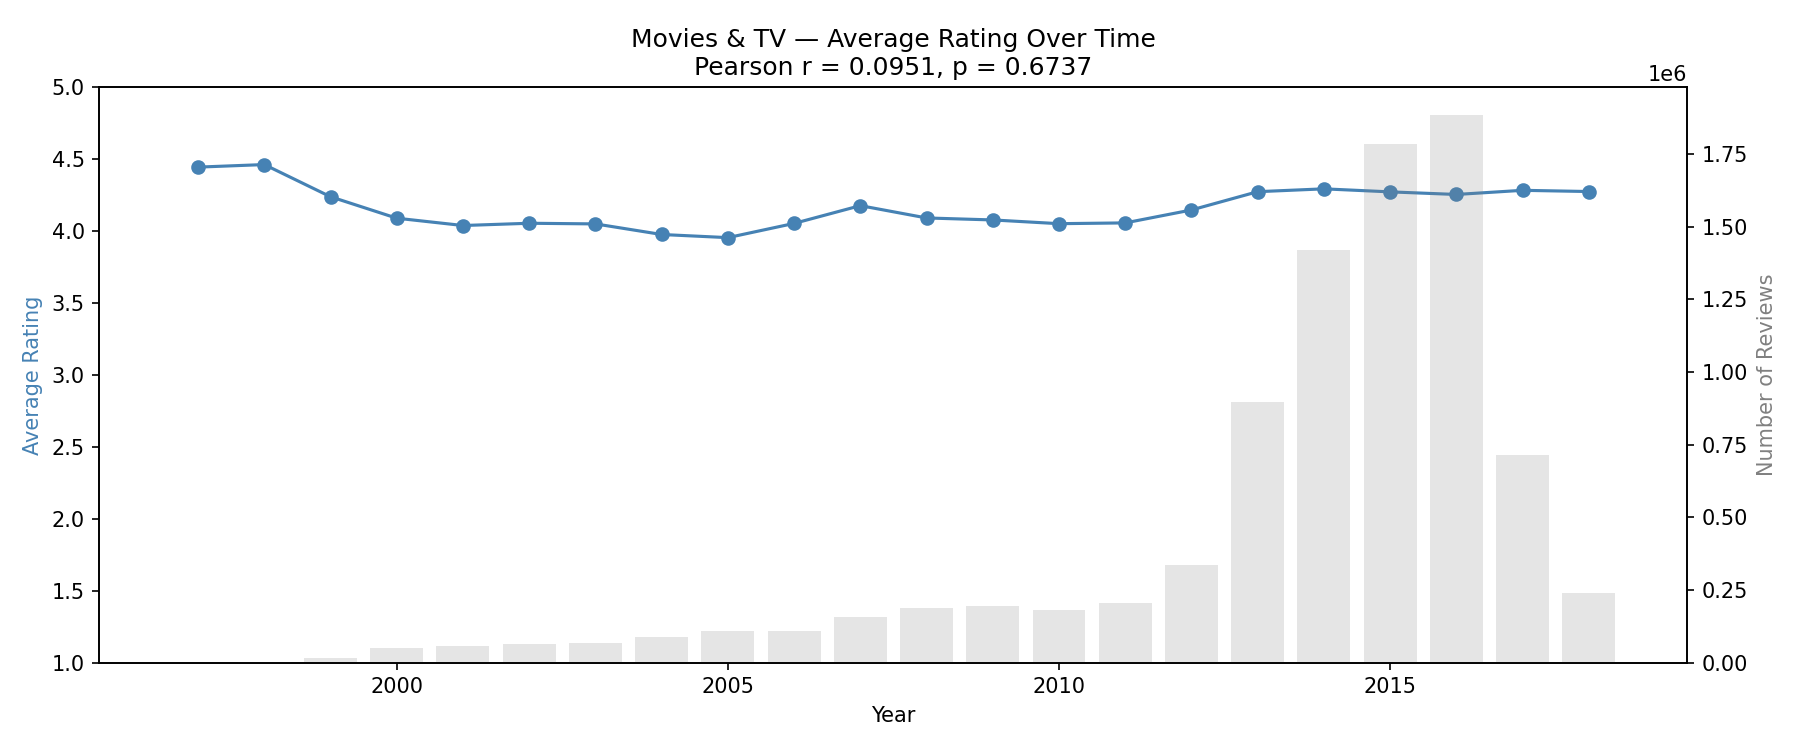
\includegraphics[width=\columnwidth]{figures/ratings_over_time.png}
\caption{Yearly mean rating (line) and yearly review count (bars, right axis), full CSV.}
\label{fig:corr_year}
\end{figure}

\begin{figure}[!t]
\centering
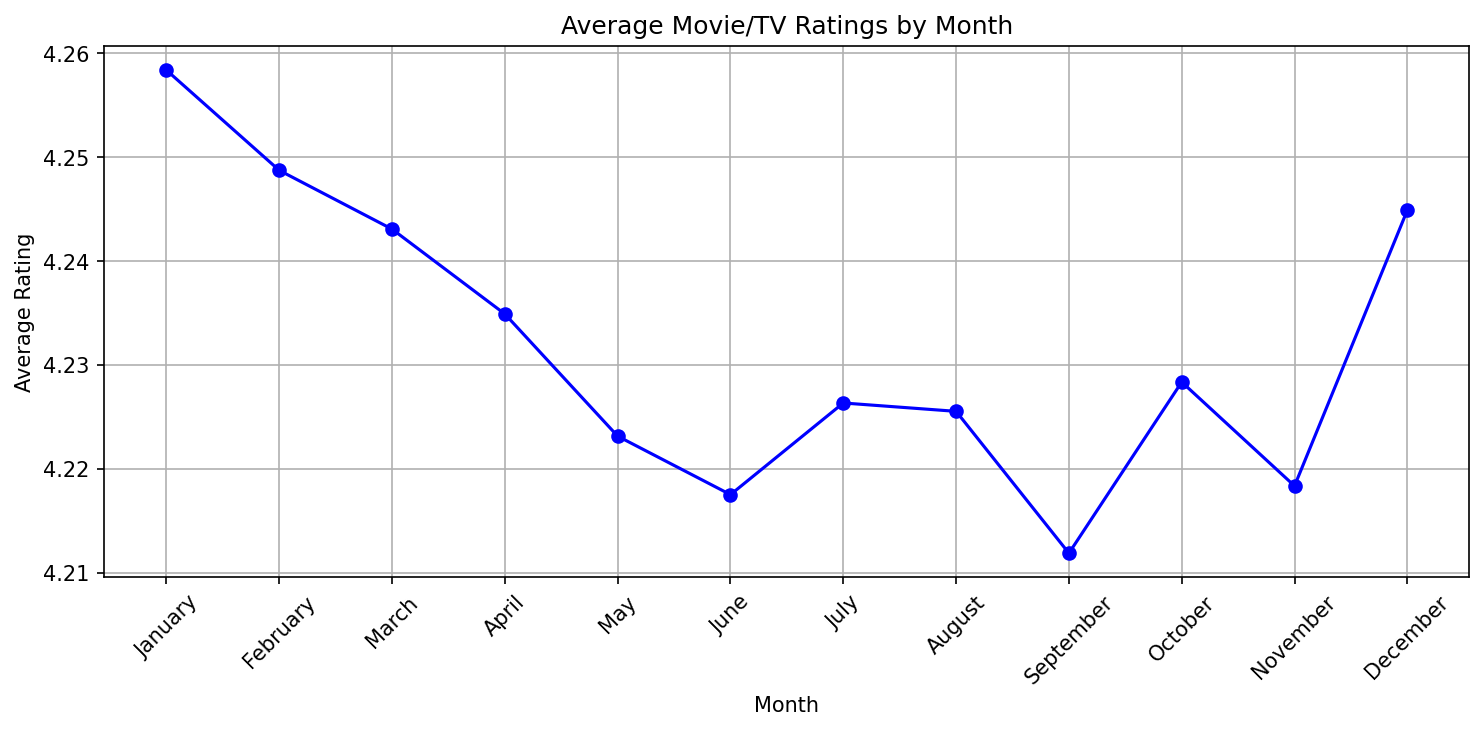
\includegraphics[width=\columnwidth]{figures/average_rating_by_month.png}
\caption{Mean rating by calendar month (all years pooled), full CSV.}
\label{fig:seasonal_month}
\end{figure}

\subsection{Popularity, disagreement, and user ``harshness'' (cohort \textbf{(F)})}
\label{sec:popularity}

Using \textbf{all} CSV rows and thresholds of at least five reviews per movie and per user (cohort \textbf{(F)}), \textbf{89{,}590} titles and \textbf{311{,}221} users entered correlation analyses (Figs.~\ref{fig:pop_mean}--\ref{fig:heavy_mix}). At this scale, even correlations near zero can attain extreme $p$-values; we therefore lead with $R^2$ and Spearman $\rho$ when judging whether popularity explains meaningful variation in average scores or disagreement.

Key coefficients include: movie review count versus mean rating---Pearson $r=0.040$ on raw counts, $r=0.098$ on $\log(1+n)$ with $R^2\approx 0.0096$, Spearman $\rho=0.067$; movie count versus within-title rating standard deviation---Spearman $\rho=-0.031$ (Fig.~\ref{fig:pop_sd}); user review count versus mean user rating---Pearson $r=-0.023$, Spearman $\rho=-0.057$. Table~\ref{tab:corr} summarizes these linear and rank associations. Heavy users (top decile of activity among filtered users; threshold $\geq 19$ reviews each) contribute \textbf{16.4\%} of rows; their overall mean rating (\textbf{4.155}) is slightly below non-heavy users (\textbf{4.248}), both on \textbf{(F)}. Within-user rating SD is slightly higher for heavy users (Mann--Whitney $p\ll 0.001$), which is consistent with mixing genuinely diverse tastes with occasional critical episodes rather than with heavy users being uniformly monotonic. On cohort \textbf{(J)}, heavy reviewers also produce longer written reviews on average. Point-biserial correlations between stars and heavy-user status on the full CSV remain numerically small ($|r|\approx 0.03$).

\begin{table}[!t]
\caption{Representative correlation summary for cohort \textbf{(F)} (CSV with movies/users each $\geq 5$ reviews).}
\label{tab:corr}
\centering
\begin{tabular}{@{}lccc@{}}
\toprule
Relationship & Pearson $r$ & Spearman $\rho$ & Interpretation \\
\midrule
Movie count vs.\ mean rating & 0.040 & 0.067 & negligible \\
Movie count vs.\ rating SD & $-0.012$ & $-0.031$ & negligible \\
User count vs.\ mean rating & $-0.023$ & $-0.057$ & negligible \\
\bottomrule
\end{tabular}
\end{table}

\begin{figure}[!t]
\centering
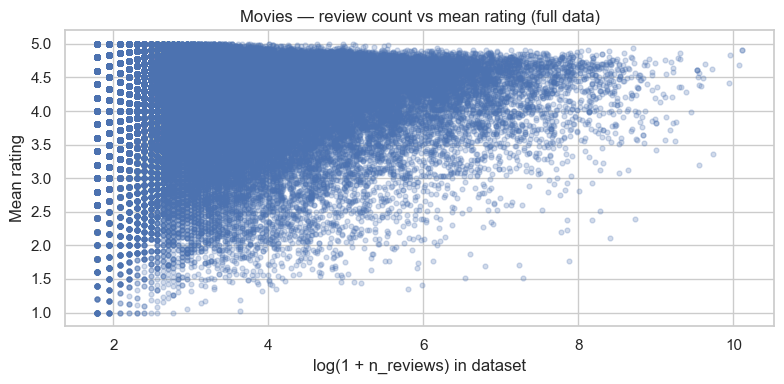
\includegraphics[width=\columnwidth]{figures/river_figure_01.png}
\caption{Movie review count versus mean rating (log-scaled activity axis), cohort \textbf{(F)}.}
\label{fig:pop_mean}
\end{figure}

\begin{figure}[!t]
\centering
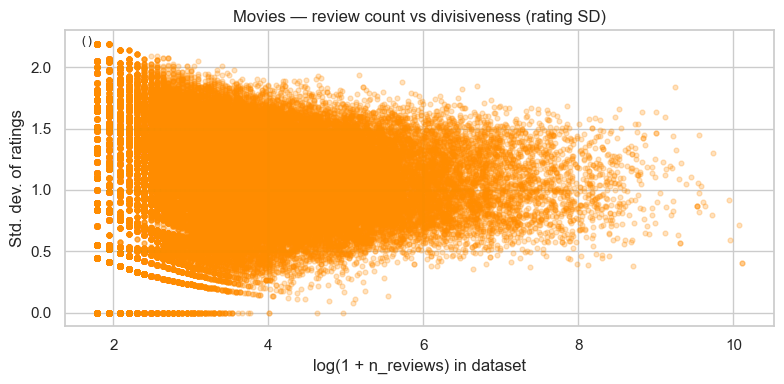
\includegraphics[width=\columnwidth]{figures/river_figure_02.png}
\caption{Movie review count versus within-title rating standard deviation, cohort \textbf{(F)}.}
\label{fig:pop_sd}
\end{figure}

\begin{figure}[!t]
\centering
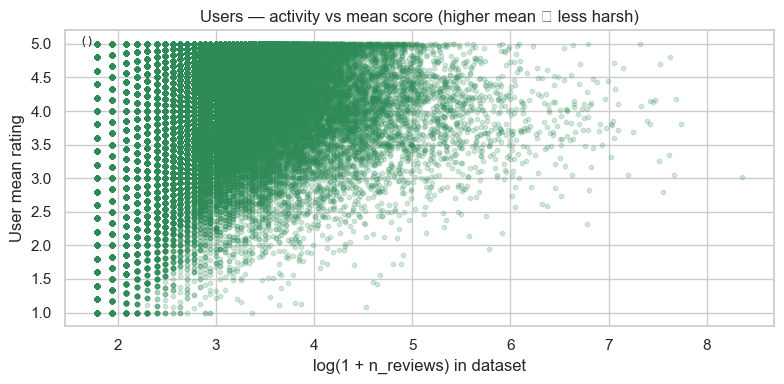
\includegraphics[width=\columnwidth]{figures/river_figure_03.png}
\caption{User review volume versus mean user rating (``harshness'' proxy), cohort \textbf{(F)}.}
\label{fig:user_mean}
\end{figure}

\begin{figure}[!t]
\centering
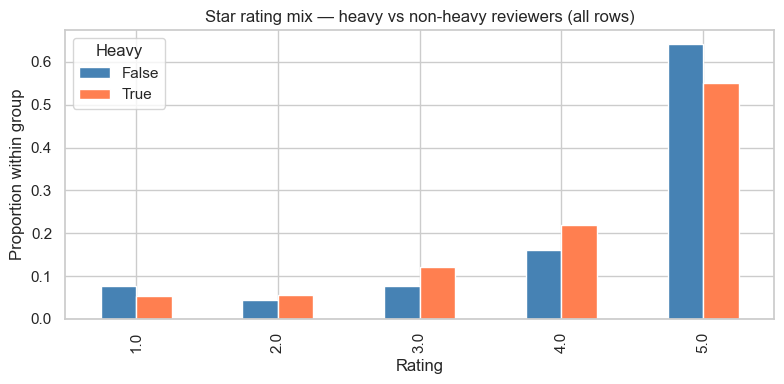
\includegraphics[width=\columnwidth]{figures/river_figure_05.png}
\caption{Share of 1--2$\star$ and 4--5$\star$ ratings for heavy versus non-heavy users.}
\label{fig:heavy_mix}
\end{figure}

\subsection{Reviewer heterogeneity and low-star concentration (cohort \textbf{(F)})}
Aggregating the CSV for users with at least five reviews (still cohort \textbf{(F)}), the mean of per-user mean ratings is \textbf{4.255} (median $4.40$, SD across users \textbf{0.721}). Only \textbf{1.13\%} of such users have overall mean $\leq 2$. Pearson $r$ between review count and mean user rating is \textbf{$-0.023$} ($p\approx 5.2\times 10^{-39}$), consistent with Fig.~\ref{fig:user_mean}; the $p$-value here mainly reflects sample size, whereas the economic and design takeaway is the near-flat relationship between activity and leniency at the user level.

Among $\leq 2\star$ reviews, concentration is sharp: the top \textbf{10\%} of users ranked by low-star volume account for \textbf{59.5\%} of all such reviews (top 20\%: 78.5\%). This pattern is important for moderation and for robust estimators: a small set of accounts contributes disproportionately to the tail of the rating distribution, so policies or models that treat reviewers as exchangeable may mis-weight rare but influential behaviors. Figs.~\ref{fig:mean_dist}--\ref{fig:lorenz} summarize the cross-user distribution of means, negative-review rates, and concentration.

\begin{figure}[!t]
\centering
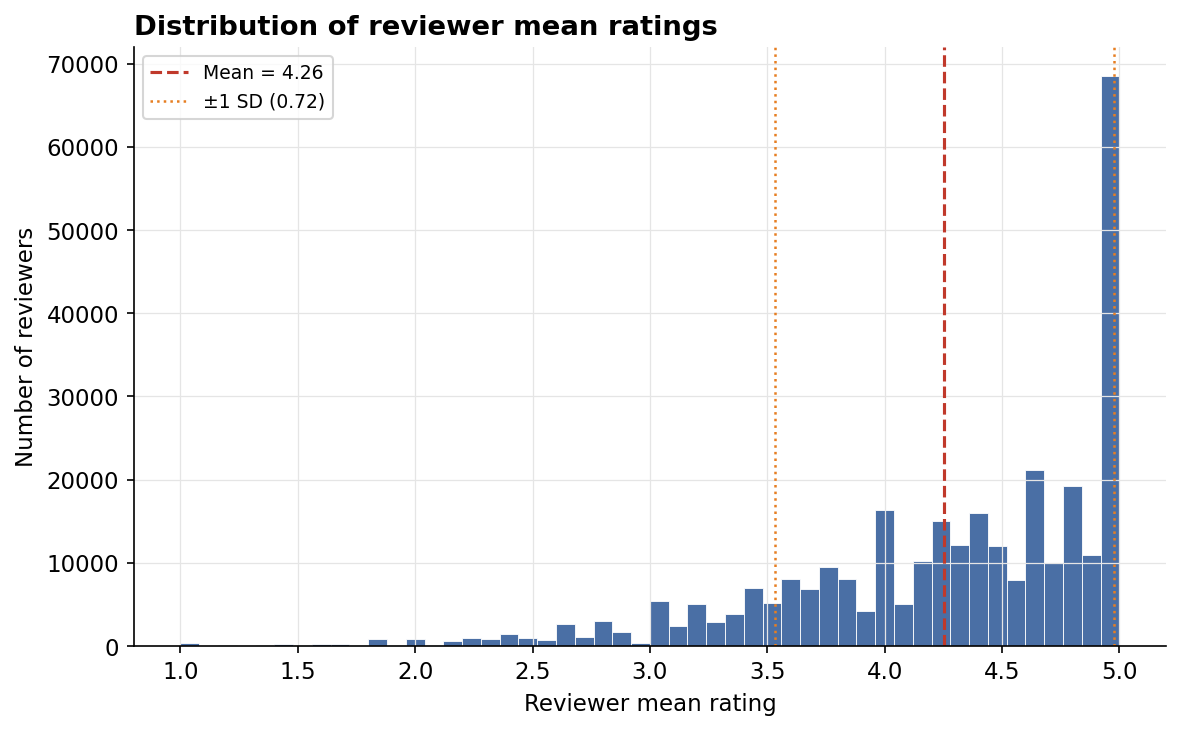
\includegraphics[width=\columnwidth]{figures/plot_mean_ratings.png}
\caption{Distribution of per-user mean ratings (users with $\geq 5$ reviews).}
\label{fig:mean_dist}
\end{figure}

\begin{figure}[!t]
\centering
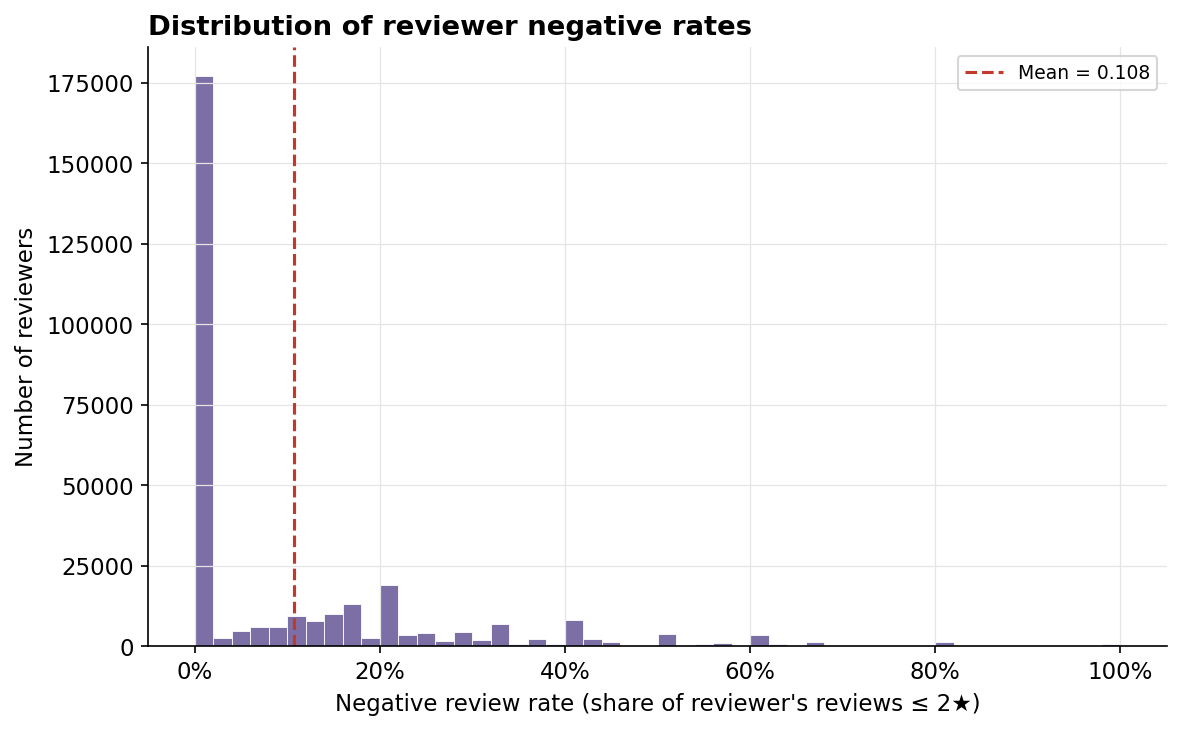
\includegraphics[width=\columnwidth]{figures/plot_negative_rates.png}
\caption{Distribution of per-user negative rate (share of reviews $\leq 2\star$).}
\label{fig:neg_rates}
\end{figure}

\begin{figure}[!t]
\centering
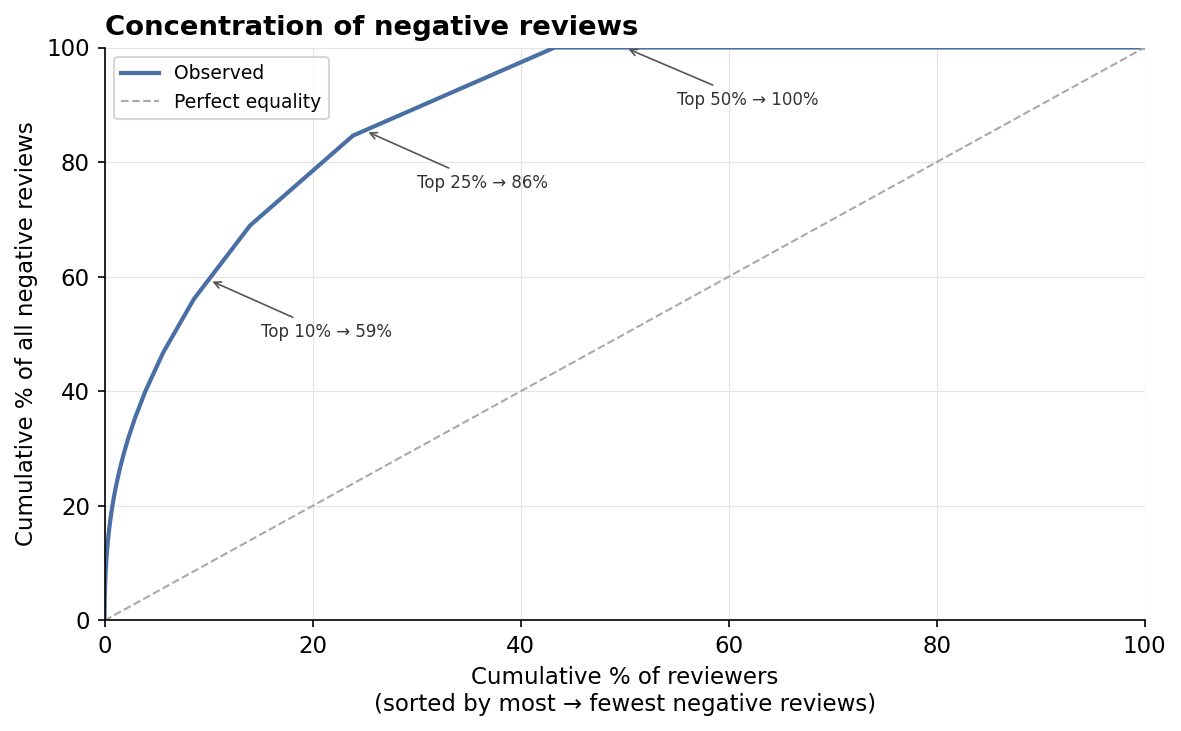
\includegraphics[width=\columnwidth]{figures/plot_concentration.png}
\caption{Cumulative share of $\leq 2\star$ reviews versus cumulative share of users sorted by low-star activity.}
\label{fig:lorenz}
\end{figure}

\subsection{Supervised ``like'' baseline (cohort \textbf{(C)})}
Encoding users and items and training a random forest on \textbf{10\%} of the CSV ($\sim$876k rows; cohort \textbf{(C)}; same seed as Appendix~\ref{app:repro}), we obtained \textbf{76.47\%} accuracy on a 20\% hold-out. In this pool, the marginal proportion of ``liked'' labels ($\geq 4$ stars) is about \textbf{79.7\%}; a naive classifier that always predicts ``liked'' therefore achieves roughly \textbf{79.7\%} accuracy. The random forest does not beat that trivial baseline, which underscores that aggregate accuracy is a poor summary here and that ID-only features do not recover minority-class structure. The minority ``dislike'' class remains harder (recall $\approx 0.15$ at precision $\approx 0.33$), reflecting imbalance and the weakness of identity-only features---consistent with the need for richer signals in real recommenders and with the fact that collaborative structure may exist but is weak when compressed into a shallow tree ensemble on encodings without careful factorization or embeddings.

\subsection{Five-core JSON: rating mass, tests, review length, and helpfulness (cohort \textbf{(J)})}
Unless noted otherwise, statistics in this subsection refer to cohort \textbf{(J)} --- the Movies \& TV \textbf{5-core} review file with \texttt{reviewText}, \texttt{vote}, and \texttt{verified} --- not to \textbf{(C)} or \textbf{(F)}.

\textbf{Rating distribution and benchmark test.} Stars pile up at the top: at least half of all ratings in this subset are \textbf{5}, and at least three quarters are \textbf{4} or \textbf{5}, so the median rating is \textbf{5} with heavy positive skew. The overall mean rating is \textbf{4.221}. For $H_0:\mu=4.0$ versus $H_1:\mu\neq 4.0$, a one-sample $t$-test yields $t\approx 350.4$ and $p<0.001$; the null is rejected, but the mean is only about \textbf{0.22} stars above the benchmark---illustrating that statistical significance does not imply a large deviation in practical terms when $n$ exceeds three million. A narrow reported 95\% CI for $\mu$ (e.g., width on the order of $10^{-3}$ stars) further shows that precision is not the same as practical importance.

\textbf{Low-star concentration (text cohort).} Many reviewers never record a rating $\leq 2$ stars in this filtered file---on the order of \textbf{176{,}000} users in team summaries---so negative signals are concentrated among a smaller set of accounts, parallel to the Lorenz-style concentration measured on the CSV (Fig.~\ref{fig:lorenz}).

\textbf{Review length.} Length distributions are strongly right-skewed: median \textbf{25} words versus mean \textbf{81.1}, so long tails inflate the mean. By rating group, \textbf{2}-star reviews tend to have the longest median length (dissatisfied users write more), while \textbf{5}-star reviews tend to have the shortest medians (brief praise).

\textbf{Correlation and regression.} Spearman $\rho$ between word count and star rating is about \textbf{$-0.191$} (weak negative monotonic link), whereas $\rho$ between length and helpful votes is about \textbf{$+0.497$} (moderate positive). Thus length aligns more with perceived usefulness than with how many stars were assigned; put differently, verbosity is not simply a proxy for satisfaction or dissatisfaction in this cohort. Fitting OLS on $\log(1+\text{helpful votes})$ with $\log(1+\text{length})$, rating, verified purchase, and year yields a positive coefficient on $\log(1+\text{length})$ (about \textbf{0.168} in team outputs): longer text remains associated with more helpful votes after controls. Verified purchases show \emph{shorter} median length than unverified reviews in tabulations; heavy reviewers write \emph{longer} text than light reviewers. Nonparametric tests on skewed margins support these comparative statements qualitatively.

One interpretation-friendly decomposition is that stars summarize global affect while length captures elaboration that other consumers find actionable; another is selection into voting---long reviews may simply be more visible or may attract readers who engage with the helpfulness buttons more often.

\section{Discussion}
Star ratings alone do not fully capture engagement: written length adds information beyond the numeric score, especially for helpfulness. Ratings are overwhelmingly high-star; means therefore cluster near 4--5 even when dispersions differ, which complicates naive interpretations of ``average satisfaction'' as an interval-scale quantity. Because $n$ is huge (millions of reviews), confidence intervals for global means are extremely narrow and tests against benchmarks such as $\mu=4.0$ \mbox{reject $H_0$ easily}; \textbf{practical significance} (effect size, business relevance) matters more than $p$-values alone. The same issue arises for tiny Pearson or Spearman correlations: statistical significance is common, while $R^2$ or rank correlations must be read for magnitude (Table~\ref{tab:corr}). In classroom terms, this is the familiar ``large $n$ problem'' of observational internet-scale data; in applied reporting, it argues for leading with plots and standardized effect summaries rather than stars-of-significance alone.

Popularity weakly tracks higher mean scores but explains under one percent of variance on the log scale; divisiveness is largely unrelated to volume. Taken together, these findings caution against treating review counts as a proxy for either average quality or controversy at the title level without richer modeling of composition (who shows up to rate blockbusters versus niche releases). Active users rate slightly lower on average, and low-star mass is concentrated among a minority of reviewers---relevant for robust aggregation and abuse monitoring, and for understanding why tail risk in ratings may be driven by idiosyncratic reviewers rather than evenly distributed dissatisfaction. The random-forest ``like'' model underperforms a constant ``liked'' prediction at the reported class balance, so aggregate accuracy by itself is misleading; metrics that stress minority-class performance (e.g., recall for low stars) are more informative. Text analyses link longer reviews to helpful votes even after controls, but helpfulness is visibility-prone and selection-laden; regression indicates association, not causation, and platform sorting algorithms likely intervene between writing and observed votes. Sparsity ($\approx 0.9998$) and filtering shrink how many entities survive minimum-activity rules, which further disconnects population-level means from the experience of infrequent raters. Unobserved confounds include genre, price, title quality, and temporal drift; any policy claim would require either richer covariates or designs that shift exposure or information sets exogenously.

\section{Conclusion}
This project combined ratings-only and text-rich Amazon Movies \& TV extracts to characterize how volume, identity-level behavior, and text length align with ratings and helpful votes. The vast majority of recorded stars are high (median \textbf{5} on 5-core); full-CSV analyses show long-tail activity, negligible popularity--score correlations, slight ``harshness'' for busy reviewers, and strong concentration of $\leq 2\star$ reviews among a subset of users. Identifier-only ``like'' prediction does not improve on a trivial majority baseline in accuracy terms, and it still misses minority ``dislike,'' underscoring that pure memorization of frequent user--item pairs is insufficient for balanced retrieval of negative sentiment. On the 5-core subset, review length is a behavioral signal partially orthogonal to stars in rank terms: it correlates weakly with rating but moderately with helpfulness and stays positive in multivariate models, suggesting that qualitative elaboration contains information not reducible to a single ordinal star click.

The overarching lesson is methodological rather than domain-specific: Amazon-scale corpora reward careful descriptive work and humility about inference. Natural extensions include stronger collaborative models (matrix factorization, sequence models), calibration for imbalanced labels, and---where feasible---designs or quasi-experiments that support causal claims beyond observational association. Because cohort \textbf{(J)} already contains \texttt{reviewText}, a natural next step is \emph{natural language processing} on that field---for example sentiment or aspect extraction, topic modeling, or neural embeddings---to test whether semantic content explains helpful votes beyond word count and to interpret \emph{why} longer reviews correlate with helpfulness. Even absent those extensions, the descriptive backbone established here clarifies which empirical patterns are genuinely robust versus artifacts of scale and sampling.

\appendices
\section{Reproducibility}
\label{app:repro}

Analyses were implemented in Python; the following artifacts refer to the course project codebase. Cohort \textbf{(S)} used a seeded subsample (e.g., \texttt{statistical\_analysis.ipynb} with fixed \texttt{TARGET\_SAMPLE\_SIZE} and seed). Cohort \textbf{(C)} temporal and seasonal figures were produced without subsampling (\texttt{correlation\_analysis.py}, \texttt{MathProjectFinal.Py}). The random-forest baseline (\texttt{recommendations.py}) draws \texttt{frac=0.1} with \texttt{random\_state=42} from \texttt{Movies\_and\_TV.csv}, label-encodes users and items, and holds out 20\% for evaluation with \texttt{random\_state=42}. Heavy-user splits and reviewer plots use \texttt{reviewer\_analysis.py} where applicable. Exact command lines depend on local paths to the McAuley release files.

\section*{Acknowledgment}
This course project uses the Amazon Review Data (2018) release \cite{mcauley2018}. Internal DATA~202 midterm and final presentation materials informed the narrative synthesis \cite{data202slides}.

\begin{thebibliography}{00}
\bibitem{mcauley2018}
J.~McAuley, ``Amazon review data (2018),'' UC San Diego. [Online]. Available: \url{https://cseweb.ucsd.edu/~jmcauley/datasets/amazon_v2/}

\bibitem{mcauley2015}
J.~McAuley, R.~Pandey, and J.~Leskovec, ``Inferring networks of substitutable and complementary products,'' in \emph{Proc.\ 21st ACM SIGKDD Int.\ Conf.\ Knowledge Discovery Data Mining}, 2015.

\bibitem{data202slides}
``DATA 202 --- Midterm and Final Presentations,'' course materials (unpublished).
\end{thebibliography}

\end{document}
